%***************************************PREAMBLE***************************************
\documentclass[a4paper,12pt]{article}

\usepackage{arxiv}

\usepackage[utf8]{inputenc} % allow utf-8 input
\usepackage[T1]{fontenc}    % use 8-bit T1 fonts
\usepackage{hyperref}       % hyperlinks
\usepackage{url}            % simple URL typesetting
\usepackage{booktabs}       % professional-quality tables
\usepackage{amsfonts}       % blackboard math symbols
\usepackage{nicefrac}       % compact symbols for 1/2, etc.
\usepackage{microtype}      % microtypography
\usepackage{lipsum}
\usepackage{float}
\usepackage{amsmath}
\usepackage{multirow}

\usepackage[utf8]{inputenc}
\usepackage{graphicx}
\usepackage{setspace}
\usepackage{tgtermes}

\title{Beat the Bookie}

\author
{
	Group Name: \texttt{Group I}\\
	Department of Electronic and Electrical Engineering\\
	University College London\\
	London, WC1E 6BT\\
}

\date{7\textsuperscript{th} January 2019}

\graphicspath{ {./images/} }

%***************************************DOCUMENT***************************************
\begin{document}
	
	\maketitle
	
	\section{Introduction}
	
	The aim of this project is to utilize past match data to make a prediction for the result of a match in the future. We will not be predicting the exact score; Instead we will be predicting if the Home team wins (“H”), the away team wins (“A”) or the game ends as a draw (“D”). The league that we will be concerned with the English Premier League (EPL).\\
	\\
	In each season of the EPL 20 domestic teams compete. For each matching, two games will be played: one at each of the two teams’ home stadiums. This will result in a team always being the “home” team and the other being the “away” team.  
	
	\section{Data Transformation and Exploration}
	
	The raw match data that was provided to us in the form of a csv file was imported and analysed thoroughly to identify any patterns and trends that could be exploited. Furthermore, the provided data will be manipulated to calculate metrics that describe the team’s performance. These metrics will act as features in the design matrix and will eventually be used to train the classifier model. 
	
	\subsection{Columns of the Provided Dataset }
	
	The provided dataset contained 22 columns. It contained data of all EPL matches from 2008 to 2019. Table 2.1 lists the columns of the provided dataset and a brief explanation as to what each quantity represents.
	
	\subsection{Number of Matches}
	
	The first thing that was observed was the number of matches played by each of the teams. It was identified that not all the teams played the same number of games from 2008 to 2019. This is most likely due to some teams getting relegated (dropping out of the EPL) and other teams being promoted (joining the EPL). This will result in the consistently strong teams who have remained in the EPL throughout having played the most games while those that have been relegated and promoted having played less games in the dataset. This is clearly visible from Fig. 2.1. The 7 teams with the most matches have played the same number of matches and are likely to have been consistently in the EPL throughout the 2008-2019 time period.  
	
	\begin{figure}[H]
		\renewcommand\thefigure{2.1}
		\centering
		
		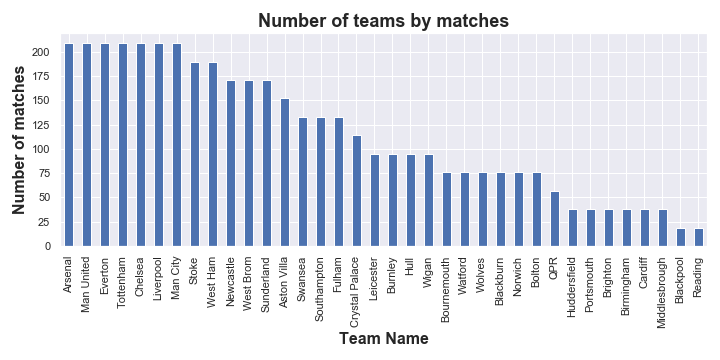
\includegraphics[scale=0.6]{num_of_matches.png}
		\caption{A count plot of the number of matches played by each of the different teams. It is clearly visible that not all teams played the same number of games.}
	\end{figure}
	
	Another quantity that was confirmed was if all possible pairings have played one another at least once in the time period of the dataset. This was found to be not the case. This is not possible due to relegation and promotion changing the list of competing teams from season to season.  
	
	\subsection{Histogram Plots of Numerical Columns}
	
	From Table 2.1.1 it is evident that most columns are integers. The distribution of each of these columns was investigated by plotting the histogram for each column. In addition to this, each bar in the histogram is split according to the full-time result (FTR). The plots are presented in Fig. 2.2 for each of the 16 integer columns in the provided dataset. It is clearly visible that most of these plots have a clear maximum either side of which the frequency drops. This could possibly indicate that these quantities may be modelled using a Poisson distribution. This is possible as each of the quantities is measured per match and therefore it is measured at a constant rate. This relationship is most clearly visible with datasets that have a large variation (i.e. have a large range). An example is the HS plot. It is clearly visible that this set of data may be modelled with a mean of around 12.\\
	\\
	\textbf{FTHG/FTAG}: The modal number of goals scored in a match by the home team is 1 whereas the modal number of goals scored in a match by the away team is 0. This loosely suggests that a team is likely to perform better at home than away, as expected.\\
	\textbf{HTHG/ HTAG}: The difference between the half time goals scored by home and away teams is a bit more subtle. The modal number of goals is 0 for both and the trends are similar.\\
	\textbf{HS/AS}: The modal class for the home shots is 12 while the modal class for the away shots is 10. This suggests a slightly lower performance when a team plays away compared to at home.\\
	\textbf{HST/AST}: By analysing the plot, the HST graph has a mean of around 4.5 while the AST graph has a mean of around 4. Which once again hints at a better performance at home.\\
	\textbf{HF/AF}: The distribution of fouls committed by the home and away teams seem to be similarly distributed.\\
	\textbf{HC/AC}: The distribution of corners is such that corners occur slightly more \\
	\textbf{HY/AY}: The approximate mean of the away plot is slightly higher than that of the home plot suggesting that teams receive more yellow cards when they play away.\\
	\textbf{HR/AR}: The occurrence of red cards was very rare, and the maximum number of red cards was 1. The histogram plot also suggests that the team that receives a red card is more likely to lose the game
	
	\begin{figure}[H]
		\renewcommand\thefigure{2.2}
		\centering
		
		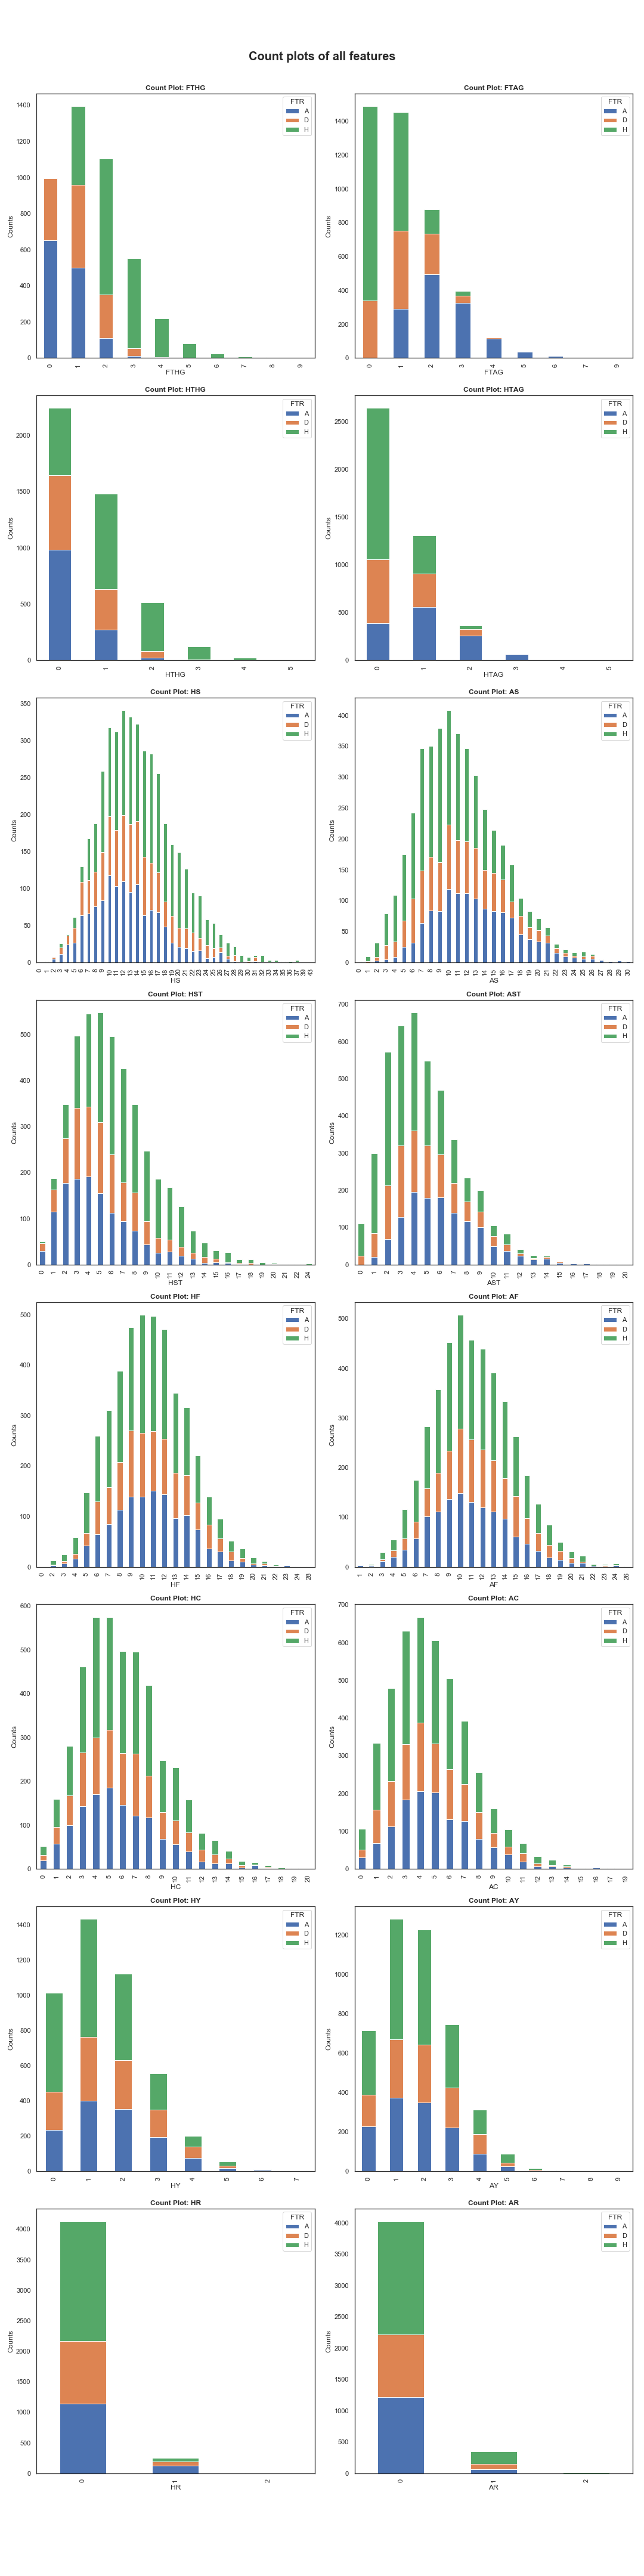
\includegraphics[scale=0.32]{count_plot_all.png}
		\caption{A count plot of the number of matches played by each of the different teams. It is clearly visible that not all teams played the same number of games.}
	\end{figure}
	
	\subsection{Analysis of Non-Numerical Columns}
	
	As shown by table 2.1.1 the non-numerical columns of the dataset are “Date”, “HomeTeam”, “AwayTeam” and “Referee”. There are 36 unique teams listed in the “HomeTeam” and “AwayTeam” columns. As expected, all teams that appear in “HomeTeam” also appear in “AwayTeam” and vice versa. As previously discussed, one season only consists of 20 competing teams. The larger number of teams in the dataset is once again due to the relegation and promotion of teams from season to season.\\
	\\
	There are also 36 unique referees across the dataset. Despite this number being equal to the number of unique teams, this is believed to be a coincidence as no specific rules on the assignment of referees that would result in this was found.\\
	\\
	The “Date” column was analysed and found that matches only occurred in months January to May and August to December. This suggests that a season of the EPL runs from August to May. This can be used to split the dataset by season and thereby find variation in team statistics by season.  
	
	\subsection{Investigation of variation in data}
	
	To investigate the spread of the data, we observe the box-plot for each of the columns containing numerical data. This is shown in fig X.X.  It can be immediately observed that there are a lot of outliers in the data. Most specifically, the HS, AS, HST and AST columns contain a lot of outlier. These outliers are most possibly caused by pairings of very strong teams against very weak teams resulting in the stronger team taking significantly more shots. The outliers in the data may result in biasing of the model as the model does not have a way to differentiate “strong” teams from “weak” teams. 
	
	\begin{figure}[H]
		\renewcommand\thefigure{2.3}
		\centering
		
		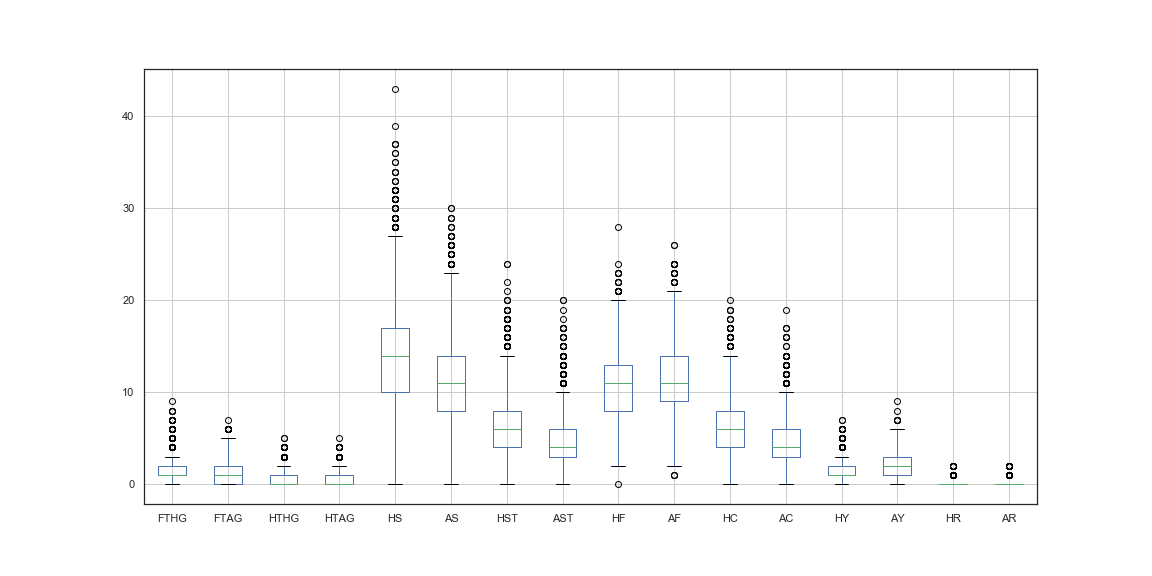
\includegraphics[scale=0.4]{raw_box_plot.png}
		\caption{A count plot of the number of matches played by each of the different teams. It is clearly visible that not all teams played the same number of games.}
	\end{figure}
	
	Thus, we consider implementing a trim function to trim out some outliers. There is a trade-off for trimming, though trimming reduce bias from outliers, the valuable available training data are lost during the process. In our case, we tried to trim all the data outside 0.2 to 0.8 percentile range, and the result is shown as the figure X.X.
	
	\begin{figure}[H]
		\renewcommand\thefigure{2.3}
		\centering
		
		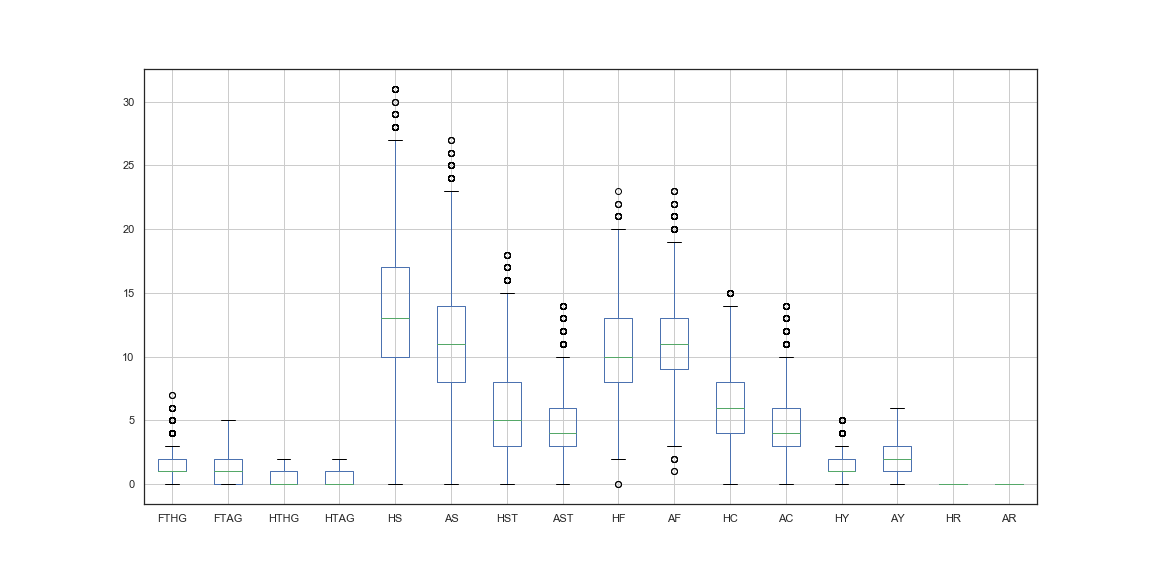
\includegraphics[scale=0.4]{trimmed_box_plot.png}
		\caption{A count plot of the number of matches played by each of the different teams. It is clearly visible that not all teams played the same number of games.}
	\end{figure}
	
	The data distribution looks more concentrated than before. Outliers, mostly outside the 0.8 percentile threshold ones are trimmed away, but when we checked about the loss of data, it was 885 out of 4180 total data, which occupied 20.5\% of our available data.\\
	\\
	Due to the relatively large portion of the training data being lost to outliers we decided to keep the outliers during the training phase. In addition to this it later occurred to us that these outliers may contain information and instead of biasing the model may separate stronger teams from weaker ones. Outliers are mainly considered in cases where the data points are expected to be within a certain range or have a specific variance. In the case of the box-plots, we are considering the data of all the teams. We also do not have equal number of data points for each team. Therefore, considering the extremities shown in the box-plot as outliers is not exactly accurate.
	
	\subsection{Correlation between columns of raw match data }
	
	To analyse the patterns in the dataset, the correlation between each of the columns was calculated. This data was represented by using a heatmap. The colours of the cells correspond to the Pearson correlation coefficient between the two columns. The most distinct feature of this heatmap is the diagonal representing correlations of 1.0. This is due to the correlation of each of the features with itself. It also follows from this that this correlation matrix is symmetrical. \\
	\\
	The half time home goals (HTHG) is strongly correlated with the full-time home goals (FTHG) with a correlation of 0.7. This also applies to the away case (HTAG and FTAG). The other strongly correlated columns are the half time result and full-time result columns (HTR and FTR). This strong correlation implies that the team that was winning at half time is likely to win the whole match as well.\\
	\\
	Another interesting correlation is that between the home corners (HC) and home shots (HS) with a correlation of 0.5. This suggests that some corners result in attempted shots at the goal for the team. Furthermore, HC also correlates with shots on target (HST) with a score of 0.4 suggesting that corners also result in shots on the target. The same applies to the away team (HC, AS and AST). However, at away matches, the correlation between AC and AST is 0.3 as opposed to 0.4 at home suggesting that corners are less likely to lead to shots on the target when a team plays away. \\
	\\
	A more obvious correlation is that the home fouls (HF) correlates with the number of yellow cards received by the home team (HY). This can easily be explained by the fact that aggressive/dangerous fouls often lead to yellow cards. \\
	\\
	It is also clearly visible that the referee column has no correlation with any of the other columns, which is indicative that it is chosen at random and does not influence the performance of either team. This relationship is expected as the job of a referee is to preside of the game from neutral point without being biased to either team.
	
	
	\begin{figure}[H]
		\renewcommand\thefigure{2.5}
		\centering
		
		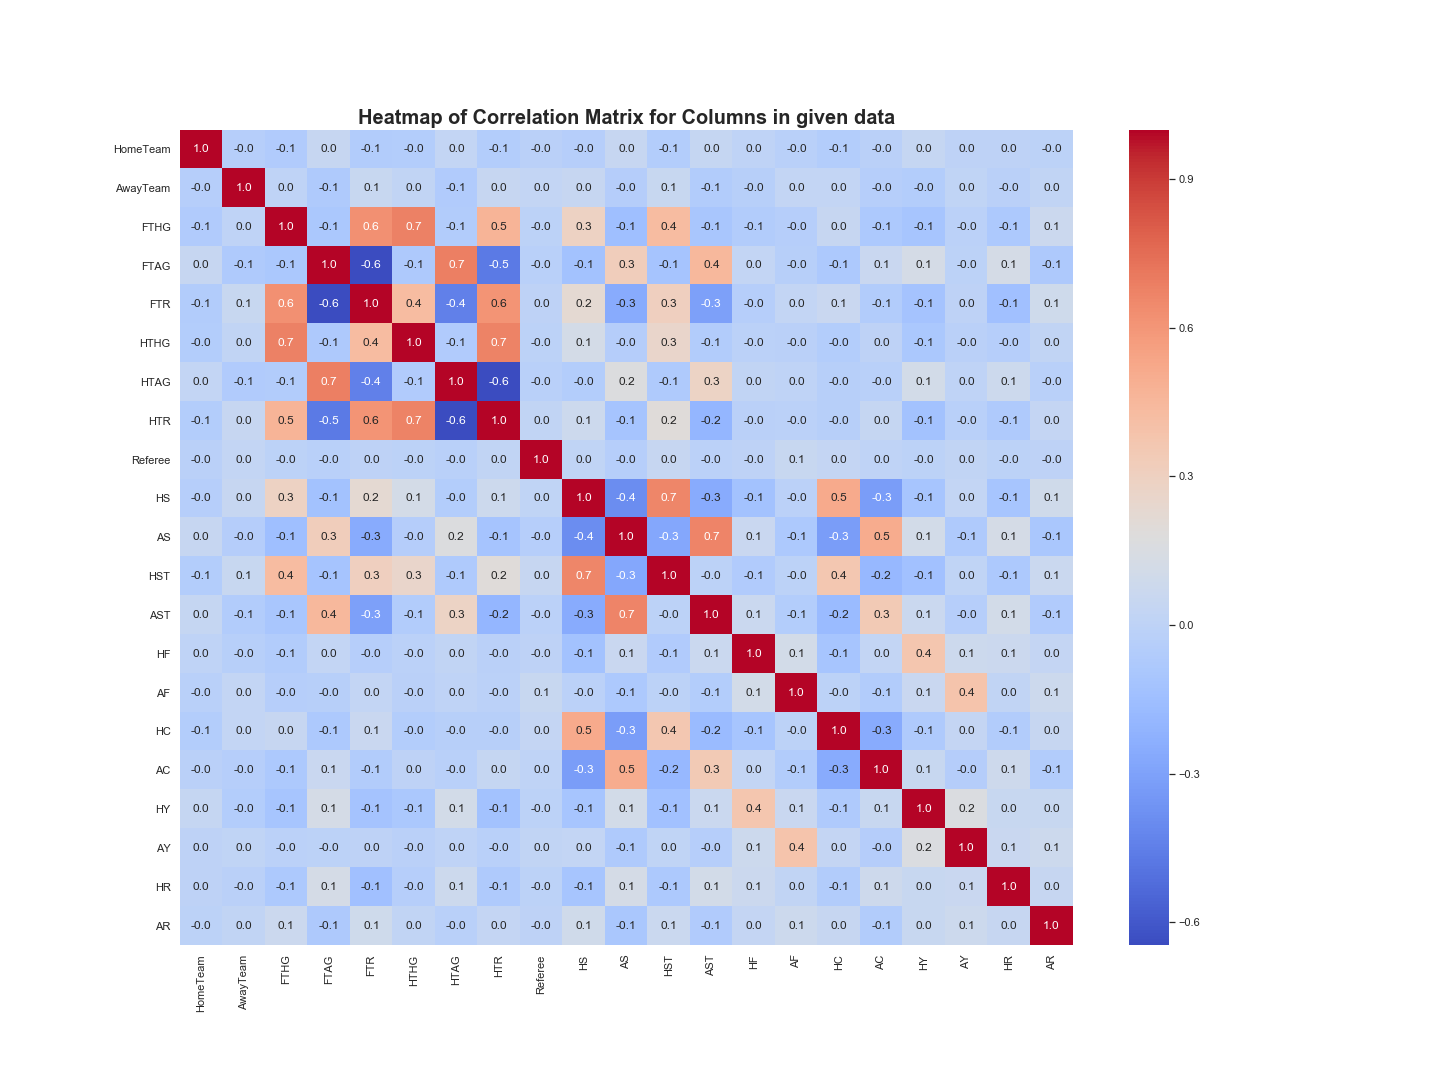
\includegraphics[scale=0.35]{raw_corr_heatmap.png}
		\caption{A count plot of the number of matches played by each of the different teams. It is clearly visible that not all teams played the same number of games.}
	\end{figure}
	

	
	\subsection{Feature Extraction}
	
	As the data in the provided dataset contains data for specific match combinations in a specific season, they do not directly contain information regarding the performance of any one team. In order to quantify the performance of a team, we devised certain metrics that are computed from the provided data which represent different qualities of each team. \\
	\\
	The first approach that was taken was to find an attacking strength and defensive strength for each team when they play away and at home. It is crucial to work out home performance scores separately to away scores as the quality of play of teams varies with where they play. In addition to attacking and defensive strength, a measure of aggressiveness of play and conversion rate were also calculated. Each of these quantities will be calculated per season to reflect the fact that teams’ performances change from season to season. It is important to note that even though these quantities change from season to season, for all matches within one season they are identical (i.e. Chelsea will have the same home attacking strength score for all matches played in the 2009/2010 season).\\
	\\
	Eight metrics are defined: Home Attacking Strength (HAS), Home Defensive Strength (HDS), Home Conversion Rate (HCON), Average Home Yellow (HY), Average Home Red (HR), Home Aggressiveness (HAGG), Away Attacking Strength (AAS), Away Defensive Strength (ADS), Away Conversion Rate (ACON), Average Away Yellow (HY), Average Away Red (HR) and Away Aggressiveness (AAGG). The equations used for computing each of these metrics is given below:
	
	
	\begin{align*}
			HAS&=\frac{\left(\frac{\text{Tot. goals scored at home}}{\text{Num. of home games played}}\right)}{\text{dataset wide avg. home goals}}           &  
			AAS&=\frac{\left(\frac{\text{Tot. goals scored away}}{\text{Num. of away games played}}\right)}{\text{dataset wide avg. away goals}}           \\
			HDS&=\frac{\left(\frac{\text{Tot. goals conceded at home}}{\text{Num. of home games played}}\right)}{\text{dataset wide avg. home conceded goals}}           &  
			ADS&=\frac{\left(\frac{\text{Tot. goals conceded away}}{\text{Num. of away games played}}\right)}{\text{dataset wide avg. away conceded goals}}           \\
			HCON&=\frac{\text{Total shots on target at home}}{\text{Total shots taken at home}}           &  
			ACON&=\frac{\text{Total shots on target away}}{\text{Total shots taken away}}           \\
			HAGG&=\frac{\left(\frac{\text{Tot. fouls commited at home}}{\text{Num. of home games played}}\right)}{\text{dataset wide avg. fouls commited}}           &  
			AAGG&=\frac{\left(\frac{\text{Tot. fouls commited away}}{\text{Num. of away games played}}\right)}{\text{dataset wide avg. fouls commited}}           \\
			HY&=\frac{\text{Total number of yellow cards received at home}}{\text{Number of home games played}}           &  
			AY&=\frac{\text{Total number of yellow cards received away}}{\text{Number of away games played}}           \\
			HR&=\frac{\text{Total number of red cards received at home}}{\text{Number of home games played}}           &  
			AR&=\frac{\text{Total number of red cards received away}}{\text{Number of away games played}}          \\
	\end{align*}
	
	The attacking strength, defensive strength, conversion rate and aggressiveness are calculated not only as an average over the whole dataset but also specifically for each season. As previously discussed, the seasons are identified by utilizing the fact that seasons start in August and run until May. By calculating these quantities by season we are able to take into consideration the fact that the performance of teams change with respect to season. \\
	\\
	Going from looking at the performance of a team over a season, we now look at the recent performance of teams against individual other teams, which are also known as head-to-head performance, where such team combinations have already played against each other before the match of interest. There are three features of interest to us in these areas: Average goals of the home team against the away team in the past n of such matches, average goals of the away team against the home team in the past n matches, and average points of the home team against the away team in the past n matches (the average points of the away team against the home team in the past n matches is included in the third variable, so is not explicitly included). We implement a function for this. A function has been implemented that takes in each individual match from the training data. In the function, the number of previous matches with the same Home Team and Away Team combination before that match is counted. If there are more or equal number of matches than a given value n, then the average goals for the away team and the average goals for the home tea, as well as the average points for the home team are calculated. If there haven’t been any prior matches with that particular combination, then the overall home and away goals average that was calculated in the beginning is given.  If the number of matches is less than n then the average is simply calculated across the matches that have been identified.
	Next, we explore extracting features relating to “form”. Form refers to a team’s recent performance I.e. if a team has been winning matches recently, then it is said to have good “form”. If a team has been winning many matches lately, then the chances that it will win further matches is likely. We can also refer to this trend of winning matches lately as a team being on a “streak”. This is something that the model will have to consider. The features we will be introducing are related to the “form” of the home team and the away team, for each match. These are the average points and goals of the home team in the last n matches and the average points and goals of the away team in the past n matches. In the case where the away and home team have not played enough to satisfy n past matches, then the results are calculated in the same way as previously. Different functions are used to obtain the streaks for the home team and the away team separately.\\
	\\
	Another feature that was added was the managers of the teams that are competing. A list of managers and their managing periods for each of the teams was obtained. From this data we were able to link each team their manager at the time of each of the matches. This data was used as a categorical feature to reflect the fact that some teams perform better under certain managers. In addition to the manager’s name the manager’s nationality was also used as a feature. \\
	\\
	Furthermore, we utilized the fact that the dates of the matches were given, to consider the weather on the date of the match. It was planned to use a historical weather API to obtain the weather on the day of the matches in the dataset and use temperate, humidity and other information relayed from the API as features for the training of the model. Unfortunately, most of the historical weather API’s were not for free access and therefore we were unable to obtain this data. \\
	\\
	A feature that we thought would influence the match was the referee of the match. However, it was observed that the referee had little correlation with the team performance. Even if the model was to use the referee as an input feature, this data is only made available on the date of the match and therefore, it won’t be available to make predictions for future matches. 
	
	
	\section{Methodology Overview}
	
	\subsection{Description of methodology}
	The posed problem is to predict which of the three classes (Home win(H), Draw(D), Away win(A)) a match falls into. As the output result is discrete and finite, this is a classification problem. The provided dataset contained statistics regarding individual matches. As previously discussed, instead of using the provided data as features, new metrics were designed to represent the performance of teams. The design of these features was discussed in the feature extraction section of the report. Using a list of Home Team and Away Team pairings as well as date, the final design matrix \textbf{X} can be formed from the \textbf{\textit{build\_X}} function. In addition to this, by looking up the result of each of these matches from the provided dataset, the label vector \textbf{y} can also be formed. Prior to training or validating the chosen models, these two quantities are split into the testing dataset and the training dataset. The chosen ratio of test to train data is 20:80. \\
	\\
	Once the features are obtained, these can be used to train models which will eventually be used to make predictions for future matches. As this is a classification problem, we are limited to classification models. The models that we chose to consider as the following:
	
	\begin{itemize}
		\item Logistic Regression (LR)
		\item K Nearest Neighbours (kNN)
		\item Random Forests (RF)
		\item Gaussian Naïve Bayes (GND
		\item Support Vector Machine (SVM)
		\item Stochastic Gradient Descent (SGD)
		\item Decision Tree Classifier (DTC)
		\item Random Forests (RFC)
		\item Extra Trees Classifier (ETC)
		\item Multi-Layer Perceptron Neural Network (MLP)
		\item Convolutional Neural Network (CNN)
	\end{itemize}

	These models were chosen purely due the fact that they can be used for multi-class classification problems. The chosen models' hyper-parameters are tuned using cross-validation techniques and eventually, their performance scores with the optimal hyper-parameters are observed.\\
	\\
	Following this, the initial design matrix is reduced in dimensionality by using principal component analysis (PCA). By utilizing PCA, correlated features (i.e. features that vary similarly and are therefore redundant) are eliminated. By doing so, the algorithm also becomes less computationally intense not only to train but also to make predictions. However, using PCA means that the final features will be a linear combination of the initial features. These features may hold little physical meaning as to the real-life performance of the team (I.e. features becomes less readable/understandable).
	Once the design matrix of reduced dimensions is obtained, the performance of the new features compared to the old features is analysed by retraining the chosen models. By comparing the scores of the models, we can choose the best performing model to make predictions on the future match pairings. 
	\subsection{Abandoned Approaches}
	One of the ideas that we explored was designing a convolutional neural network with custom layers. This was attempted by utilizing the pyTorch library. Unfortunately, we were not able to train the model to provide meaningful predictions. The outputs of the CNN suggested an equal probability that the game would win in a home win, draw or away win; which is the same as guessing. The attempted architecture of the designed network is given in table X.X.
	
	\begin{table}[H]
		\centering
		\begin{tabular}{@{}lll@{}}
			\toprule
			Layer Type & Output Shape & Number of Parameters \\ \midrule
			Linear-1   & [-1,1,36]    & 2628                 \\
			Linear-2   & [-1,1,36]    & 1332                 \\
			Linear-3   & [-1,1,18]    & 666                  \\
			Linear-4   & [-1,1,18]    & 342                  \\
			Linear-5   & [-1,1,9]     & 171                  \\
			Linear-6   & [-1,1,3]     & 30                   \\ \bottomrule
		\end{tabular}
	\end{table}
	
	\section{Model Training \& Validation}
	
	The chosen models have previously been listed. These were chosen purely as they are suitable for the multi-class classification problem that we are posed with. During the training stages, the training dataset is utilized. The testing dataset is only used to compute the performance of the models once they have been completely trained and had their hyper-parameters tuned. This ensures that there is not contamination in the training and testing datasets.\\
	\\
	As previously discussed, we know that the posed problem is a multi-class classification problem. The previously mentioned models are initially trained with scikit learn’s \textbf{\textit{cross\_validate}} function. This function evaluates the metrics by using cross validation. These are used to get a feel for the rough accuracy of the models. This was mainly used to see how well the engineered features were performing during developing stages. \\
	\\
	In order to quantify how good these models perform, we need evaluation functions. The previously mentioned \textbf{\textit{cross\_validate}} function can return multiple scoring metrics regarding the training performance: accuracy, precision, f1 score and ROC AUC score. These metrics are initially computed on the model with default hyper-parameters with the training dataset. Following this, the hyper-parameters of the model are tuned. This is done by setting up a parameter dictionary for each model. This dictionary consists of keys that correspond to the different hyper-parameters of the model. The values assigned to this dictionary key represents the different values of the specific hyper-parameters that are to be tried. This parameter grid is then utilized by the \textbf{\textit{RandomizedSearchCV}} function as well as \textbf{\textit{GridSearchCV}}. Initially the hyper-parameters are roughly tuned by utilizing the \textbf{\textit{RandomizedSearchCV}}. During this phase the values in the parameter grid have a large range and have many entries. The \textbf{\textit{RandomizedSearchCV}} will not attempt all combinations but random combinations and it is proven that it will converge roughly toward the optimally performing parameters. Once a rough idea for the range of the optimal parameters is obtained, the parameter grid is altered to be more specific with a lower range and less values. Following this, the parameter grid is utilized by \textbf{\textit{GridSearchCV}}. This function tries every combination of the different parameter values and returns the best performing combination. \\
	\\
	To visualize the performance of the model with the best hyper-parameters the confusion matrix of the performance of the model on the test data set is also plotted. This is a nice way to visualize correctly labelled and incorrectly labelled data points. It also helps to identify any biasing in the way the model makes predictions. In addition to the confusion matrix, the accuracy, precision and recall of the model is also recorded for comparison later.\\
	\\
	Once the trained and tuned model is obtained, the 15 most important features are listed. This will help during the feature selection process. In addition, it will help us identify any useless features with no meaningful contribution to the final prediction. However, this attribute is not available to all models. The GNB classifier, kNN classifier as well as the MLP classifier do not have this attribute.
	Once this has been done for all the chosen models, the scores of the performance on the test set are considered and the model performance is evaluated. Before the best model is chosen, the dimensionality of the problem is reduced. Currently, the number of input features stands at 46. By using PCA, we aim to reduce the number of features and thereby reduce the complexity of the model which will mean that it will be quicker not only to train but also to make predictions.\\
	\\
	After having obtained the design matrix with the reduced number of dimensions, the models are re-trained using the same process as described above. The final scores are considered and the best score amongst the models trained before and after dimensionality deduction is selected. This model is then used to make the final prediction on the future matches. 
	
	
	\section{Results}
	
	As previously discussed, multiple models were considered during out approach. To pick and choose the best performing model we evaluated the performance of each of the models as mentioned in \S 4. Having carried out the training procedure, the following performance scores were obtained:
	
	\begin{table}[H]
		\centering
		\begin{tabular}{@{}lllllllll@{}}
			\toprule
			\multicolumn{1}{l|}{\multirow{2}{*}{Model}} & \multicolumn{4}{l|}{Before PCA}                                                                               & \multicolumn{4}{l|}{After PCA}                                                                                \\ \cmidrule(l){2-9} 
			\multicolumn{1}{l|}{}                       & \multicolumn{1}{l|}{Acc} & \multicolumn{1}{l|}{F1} & \multicolumn{1}{l|}{ROC\_AUC} & \multicolumn{1}{l|}{Mean} & \multicolumn{1}{l|}{Acc} & \multicolumn{1}{l|}{F1} & \multicolumn{1}{l|}{ROC\_AUC} & \multicolumn{1}{l|}{Mean} \\ \midrule
			LR                                          & 0.492178                 & 0.433495                & 0.637173                     & \textbf{0.520949}                  & 0.482496                 & 0.439982                & 0.63767                      & \textbf{0.520049}                  \\
			SGD                                         & 0.520371                 & 0.375741                & 0.646132                     & \textbf{0.514082}                  & 0.519231                 & 0.381855                & 0.636217                     & \textbf{0.512434}                  \\
			GNB                                         & 0.496444                 & 0.445201                & 0.651078                     & \textbf{0.530907}                  & 0.509831                 & 0.384703                & 0.637136                     & \textbf{0.510557}                  \\
			KNN                                         & 0.474514                 & 0.416929                & 0.601184                     & \textbf{0.497542}                  & 0.471661                 & 0.410997                & 0.594389                     & \textbf{0.492349}                  \\
			SVM                                         & 0.514101                 & 0.387864                & 0.620013                     & \textbf{0.507326}                  & 0.51581                  & 0.391111                & 0.618976                     & \textbf{0.508632}                  \\
			DTC                                         & 0.491032                 & 0.3695                  & 0.603392                     & \textbf{0.487975}                  & 0.446024                 & 0.289807                & 0.529611                     & \textbf{0.421814}                  \\
			RFC                                         & 0.525498                 & 0.421603                & 0.650564                     & \textbf{0.532555}                  & 0.522082                 & 0.40612                 & 0.642205                     & \textbf{0.523469}                  \\
			ETC                                         & 0.506134                 & 0.421658                & 0.641313                     & \textbf{0.523035}                  & 0.506985                 & 0.394644                & 0.628026                     & \textbf{0.509885}                  \\
			MLP                                         & 0.522078                 & 0.398586                & 0.63955                      & \textbf{0.520071}                  & 0.524926                 & 0.391324                & 0.643869                     & \textbf{0.52004}                   \\
			XGB                                         & 0.511819                 & 0.432949                & 0.644367                     & \textbf{0.529712}                  & 0.520083                 & 0.422649                & 0.642773                     & \textbf{0.528502}                  \\ \bottomrule
		\end{tabular}
	\end{table}
	
	To help choose the best model from the pool of trained models, we decided to use the average of the accuracy, f1 score and roc\_auc score. The chosen method of calculating the roc\_auc is one vs rest, meaning that when one class is considered, the remaining classes are of the same class and then the roc\_auc is that of a binary classification problem.\\
	\\
	The difference in the mean scores for the different models do not vary much, though it is clear to see that the model with the highest average performance scores is the random forests classifier prior to being subject to dimensionality reduction due to PCA. 
	
	\section{Final predictions on Test Set}
	
	The final predictions are done on the future match pairings. These are matches that will take place on the 11th January 2020. There are 10 different pairings for which we are to predict outcomes. The csv file containing the date, home team and away team is imported and by utilizing the \textbf{\textit{build\_X}} function, the features for the match are computed. If the best model had been one that was achieved with PCA, the input feature matrix would also be modified accordingly by utilizing PCA. However, in out case the best performing model was prior to dimensionality reduction. This matrix of features is then fed into the chosen best model to make predictions. \\
	\\
	An issue that we did encounter was the fact that the prediction pairings had a team that had recently been promoted to the premier league: Sheffield United. This was an issue as no data was present for the team at the point. To overcome this, the data was updated to include data from the current season as well. Even though this is not ideal, as only little match data is available on Sheffield United, it is better than having no data.\\
	\\
	The final predictions that we obtained from the model for the match pairings are as follows:
	
	\begin{table}[H]
		\centering
		\begin{tabular}{@{}llll@{}}
			\toprule
			Date      & Home Team        & Away Team   & Result \\ \midrule
			11-Jan-20 & Bournemouth      & Watford     &        \\
			11-Jan-20 & Aston Villa      & Man City    &        \\
			11-Jan-20 & Chelsea          & Burnley     &        \\
			11-Jan-20 & Crystal Palace   & Arsenal     &        \\
			11-Jan-20 & Everton          & Brighton    &        \\
			11-Jan-20 & Leicester        & Southampton &        \\ \cmidrule(r){1-3}
			11-Jan-20 & Man United       & Norwich     &        \\
			11-Jan-20 & Sheffield United & West Ham    &        \\
			11-Jan-20 & Tottenham        & Liverpool   &        \\
			11-Jan-20 & Wolves           & Newcastle   &        \\ \bottomrule
		\end{tabular}
	\end{table}


	\section{Conclusion}
	
	Overall, the quality of the models was fair. We were able to achieve testing accuracies of consistently around 50\%. The engineered features made logical sense and seemed to positively impact the model performance. It was interesting to see that while some models benefited from dimensionality reduction via PCA, others saw their performance drop. Despite this, the change in performance was marginal and the major reason for utilizing PCA was for decreasing the complexity of the final model, which in the end was not required. In hind-sight, the number of features that we initially started off with was 42. Relative to other models in the machine learning paradigm, this is a low number and dimensionality reduction was not a necessity. \\
	\\
	To further improve the performance of the model a few considerations could be made. A factor that greatly influences team performance especially in the EPL is the squad of the team as well as player stats of the squad. This could possibly shine light into characteristics such as player chemistry. In addition to this, by utilizing player statistics, more accurate metrics for defensive and attacking strength can be obtained. This approach was attempted but not pursued greatly due to the time constraint of the assignment.
	
	
	\section*{Appendix}
	
	\subsection*{Appendix 1: Columns of provided dataset}
	\begin{table}[H]
		\centering
		\begin{tabular}{@{}lll@{}}
			\toprule
			Column   & Description                                    & Data Type                                                                \\ \midrule
			Date     & The date the match was played                  & \begin{tabular}[c]{@{}l@{}}String in Format:\\ “YYYY-MM-DD”\end{tabular} \\
			HomeTeam & The team playing at home                       & String                                                                   \\
			AwayTeam & The team playing away                          & String                                                                   \\
			FTHG     & Goals scored by the home team at full time     & Integer                                                                  \\
			FTAG     & Goals scored by the away team at full time     & Integer                                                                  \\
			FTR      & Full-Time result of the match                  & One of “H”, ”A” or D                                                     \\
			HTHG     & Goals scored by home team at half time         & Integer                                                                  \\
			HTAG     & Goals scored by away team at half time         & Integer                                                                  \\
			HTR      & Half-Time result of the match                  & One of “H”, ”A” or D                                                     \\
			Referee  & The name of the referee for the match          & String                                                                   \\
			HS       & The number of shots taken by the home team     & Integer                                                                  \\
			AS       & The number of shots taken by the away team     & Integer                                                                  \\
			HST      & The number of shots on target by the home team & Integer                                                                  \\
			AST      & The number of shots on target by the away team & Integer                                                                  \\
			HF       & The number of fouls committed by the home team & Integer                                                                  \\
			AF       & The number of fouls committed by the away team & Integer                                                                  \\
			HC       & The number of corners by the home team         & Integer                                                                  \\
			AC       & The number of corners by the away team         & Integer                                                                  \\
			HY       & The number of yellow cards to the home team    & Integer                                                                  \\
			AY       & The number of yellow cards to the away team    & Integer                                                                  \\
			HR       & The number of red cards to the home team       & Integer                                                                  \\
			AR       & The number of red cards to the away team       & Integer                                                                  \\ \bottomrule
		\end{tabular}
	\end{table}

	\subsection*{Appendix 2: Dependencies of the final code}
	
	\begin{itemize}
		\item os
		\item warnings
		\item requests
		\item Beautiful Soup 4
		\item time
		\item dateutil
		\item multiprocessing
		\item numpy
		\item pandas
		\item seaborn
		\item scikit learn
		\item matplotlib
	\end{itemize}
	
\end{document}
